\chapter{Results and Analysis}
\label{ch:results}

This chapter reports the forecasting experiment and reads its outcome honestly.
The model of Chapter~\ref{ch:arch} is trained and evaluated under the
leave-one-active-region-out protocol (\S\ref{sec:setup}); the forecasts on a
held-out region are shown and quantified (\S\ref{sec:forecast}); and the result
is then interpreted, separating the genuine skill of the model from the
persistence that a smoothly evolving field affords for free
(\S\ref{sec:discussion}).

\section{Experimental setup}
\label{sec:setup}

The encoder--forecaster is trained on the pooled gap-aware windows of $26$
active regions and evaluated on a single held-out region, HARP~11930, that it
never sees during training. The noisy region flagged in \S\ref{sec:data} is
excluded from every split. Each cube contributes only windows whose ten input
and four target frames are consecutive in real time at the nominal $12$-minute
cadence, so no window straddles an acquisition gap; this yields $2{,}784$
training windows and $61$ held-out windows. All frames are the accumulated total
winding of Eq.~\eqref{eq:cumsum}, asinh-normalised and low-passed onto a fixed
$88\times132$ grid.

The model is a three-layer ConvLSTM encoder--forecaster ($3.3$~million
parameters, hidden width $96$), trained for $48$ epochs with Adam, a cosine
learning-rate decay, and gradient-norm clipping, forecasting $t_{\text{out}}=4$
frames ($48$~minutes) from $t_{\text{in}}=10$ history frames ($120$~minutes). The
reference against which it is judged is the \emph{persistence} forecast---copying
the last observed frame forward---which is the natural zero-skill baseline for a
strongly autocorrelated field and the fallback the residual parameterisation of
Eq.~\eqref{eq:residual} is built around. Skill is defined as the fractional
reduction in mean absolute error relative to persistence,
\begin{equation}
  \text{skill} \;=\; 1 - \frac{\mathrm{MAE}_{\text{model}}}{\mathrm{MAE}_{\text{persistence}}}.
  \label{eq:skill}
\end{equation}

\section{Forecasting the held-out active region}
\label{sec:forecast}

\paragraph{Headline result.}
On the held-out region HARP~11930---never seen in training---the ConvLSTM
forecasts the accumulated winding field over a $48$-minute horizon with a mean
absolute error of $\mathbf{0.0106}$, against $\mathbf{0.0117}$ for the
persistence baseline: a skill of $\mathbf{+9.3\%}$ by Eq.~\eqref{eq:skill},
measured over all $61$ gap-aware windows of the region. The model therefore
generalises across active regions and improves on the trivial forecast.
Table~\ref{tab:results} states these numbers together.

\begin{table}[t]
\centering
\caption[Forecast results]{\textbf{Forecast accuracy on the held-out active
region.} Mean absolute error (normalised units) over all $61$ gap-aware windows
of HARP~11930, for the ConvLSTM and for the persistence baseline, with the skill
of Eq.~\eqref{eq:skill}. The model was trained only on the other $26$ regions.}
\label{tab:results}
\begin{tabular}{@{}lc@{}}
\toprule
Forecaster (held-out HARP~11930, $48$-min horizon) & MAE \\
\midrule
Persistence (copy last observed frame)             & $0.0117$ \\
ConvLSTM encoder--forecaster (this work)           & $\mathbf{0.0106}$ \\
\midrule
\textbf{Skill over persistence} & \multicolumn{1}{r}{$\mathbf{+9.3\%}$} \\
\bottomrule
\end{tabular}
\end{table}


\paragraph{Frame-by-frame verification.}
A forecast is judged not by how good the prediction looks but by how it differs
from the truth. Figure~\ref{fig:triptych} places the two side by side at every
lead time: the top row is the prediction, the middle row the observation at the
same instant, and the bottom row their difference. Prediction and truth are
near-identical at the large scale. The residuals, on the expanded scale of the
bottom row, are small (a few per cent of the field amplitude) and---tellingly---
\emph{structured}: they are not spread uniformly but concentrate in fine specks
along the boundaries between the opposed winding lobes, precisely where the field
has its sharpest gradients. This is the fine-scale content that
\S\ref{sec:data} identified as temporally incoherent: the model reproduces the
smooth envelope and errs only on the unpredictable detail, and the error grows
frame by frame as that detail decorrelates.

\begin{figure}[t]
\centering
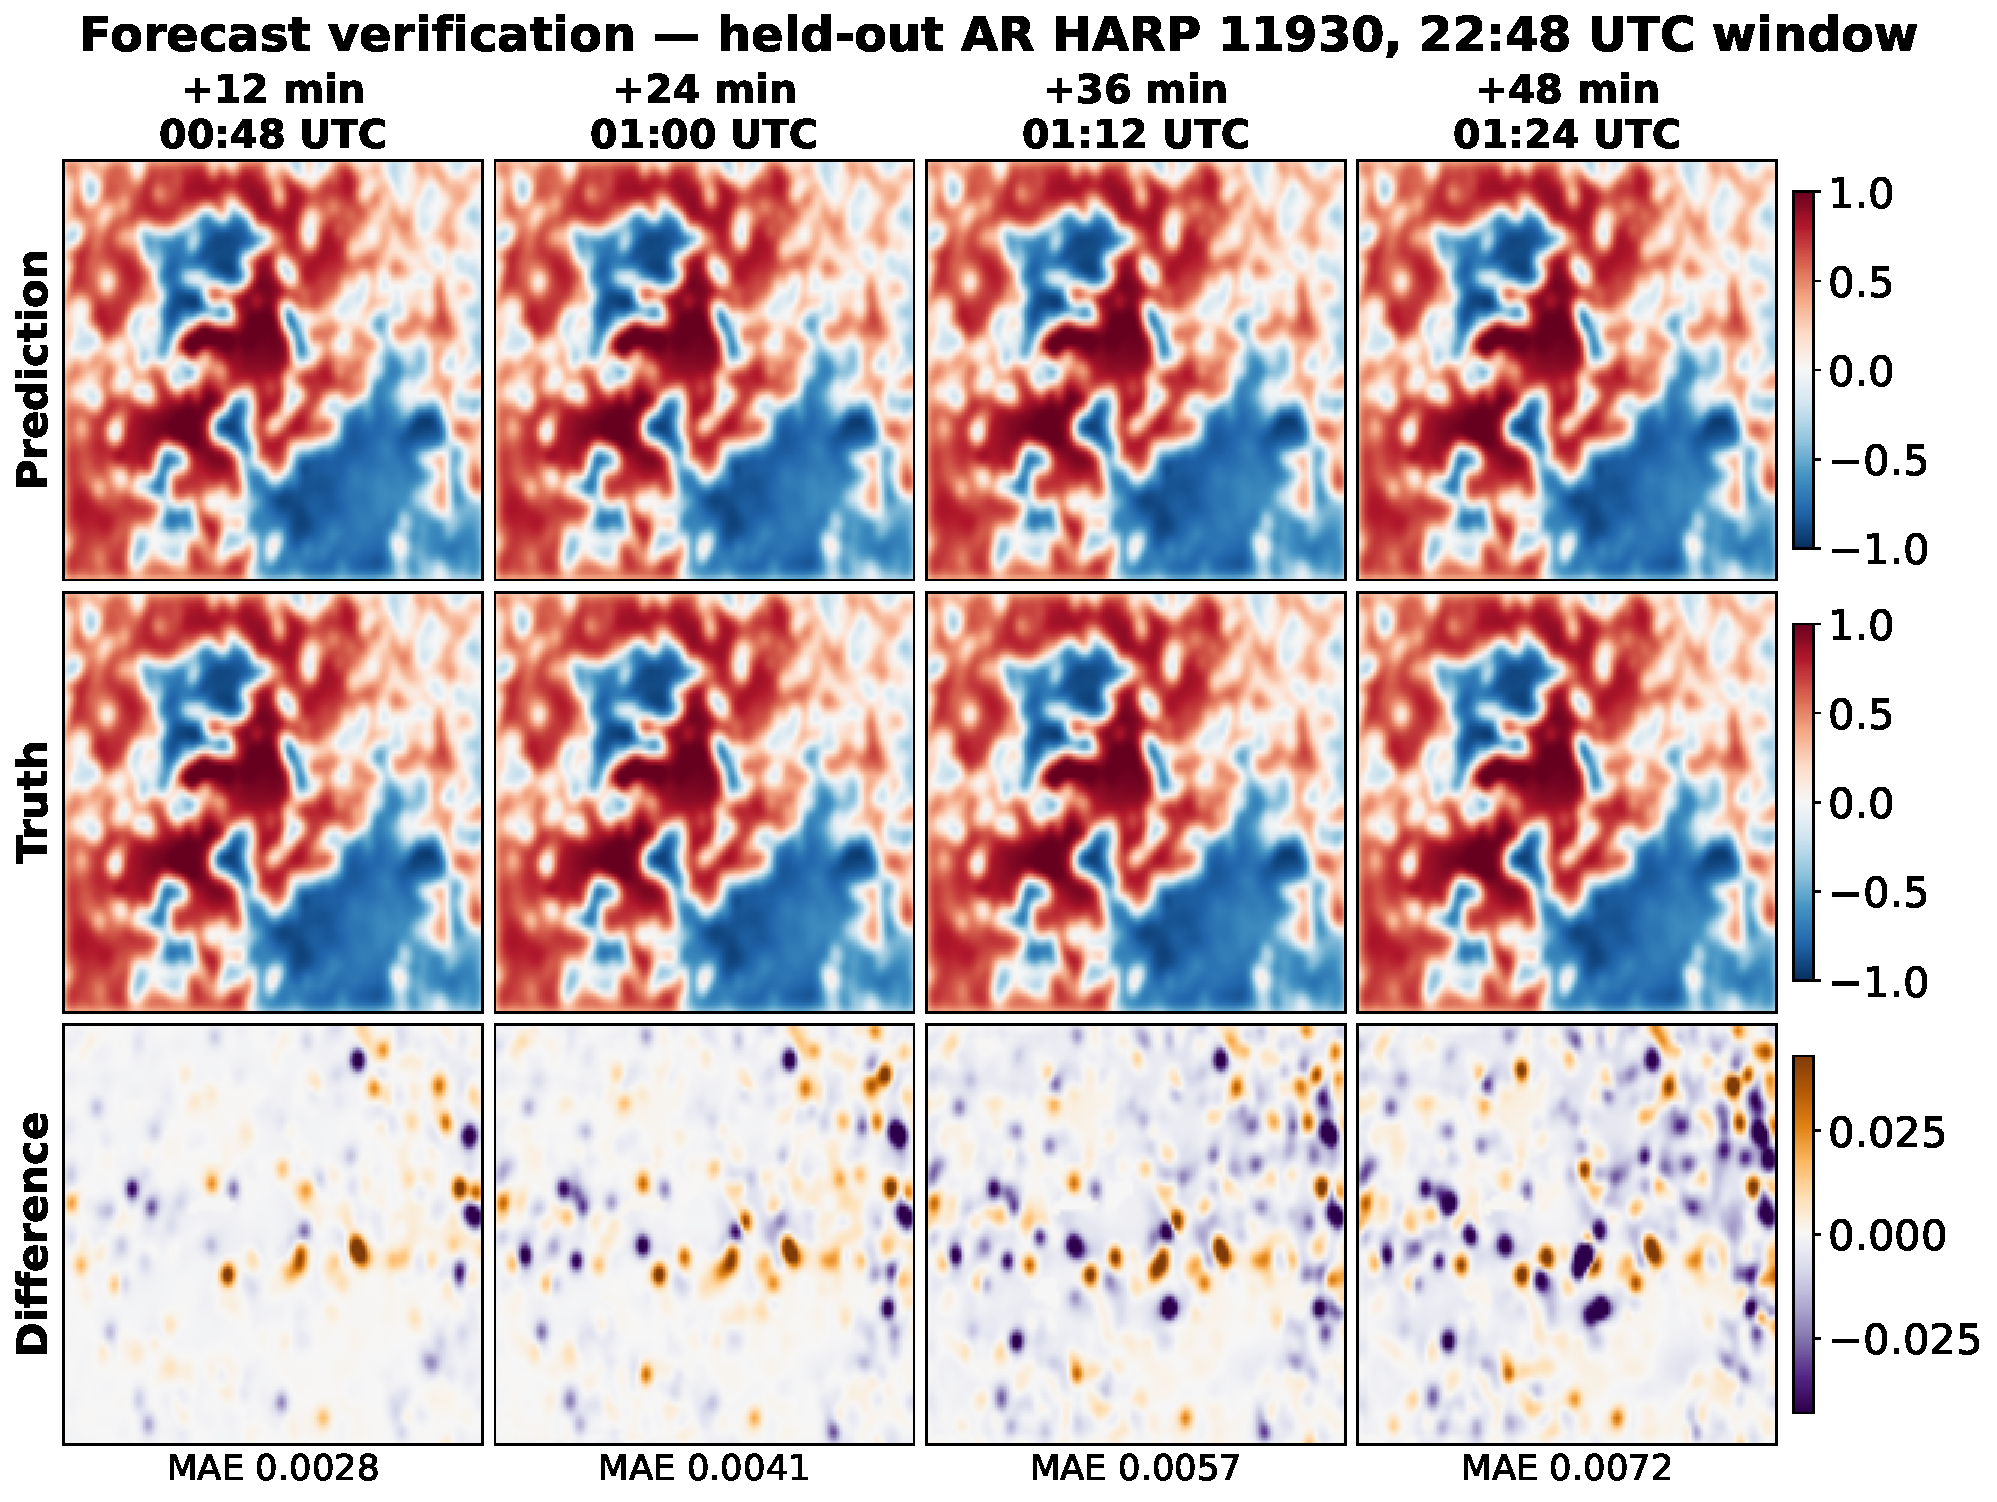
\includegraphics[width=\textwidth]{figures/fig_triptych.pdf}
\caption[Forecast verification]{\textbf{Frame-by-frame verification on the
held-out region.} For one window of HARP~11930: predicted field (top), observed
field (middle), and their difference (bottom, on an expanded colour scale) at
lead times $+12$ to $+48$~minutes. Errors are small, grow with lead time (per-frame
MAE annotated), and localise along the sharp-gradient boundaries between winding
lobes---the fine structure that cannot be forecast.}
\label{fig:triptych}
\end{figure}

\paragraph{How error grows with lead time.}
Figure~\ref{fig:horizon} traces the mean absolute error, averaged over all $61$
held-out windows, as a function of lead time, for the model and for persistence.
Both grow as the field decorrelates, but their relationship is informative: at
$+12$~minutes the two coincide---over a single step the accumulated field barely
changes, so nothing beats copying it---while at every later step the model pulls
below persistence, the margin widening to $+48$~minutes. The model has therefore
learned genuine short-term dynamics, and its advantage is largest exactly where
persistence degrades fastest.

\begin{figure}[t]
\centering
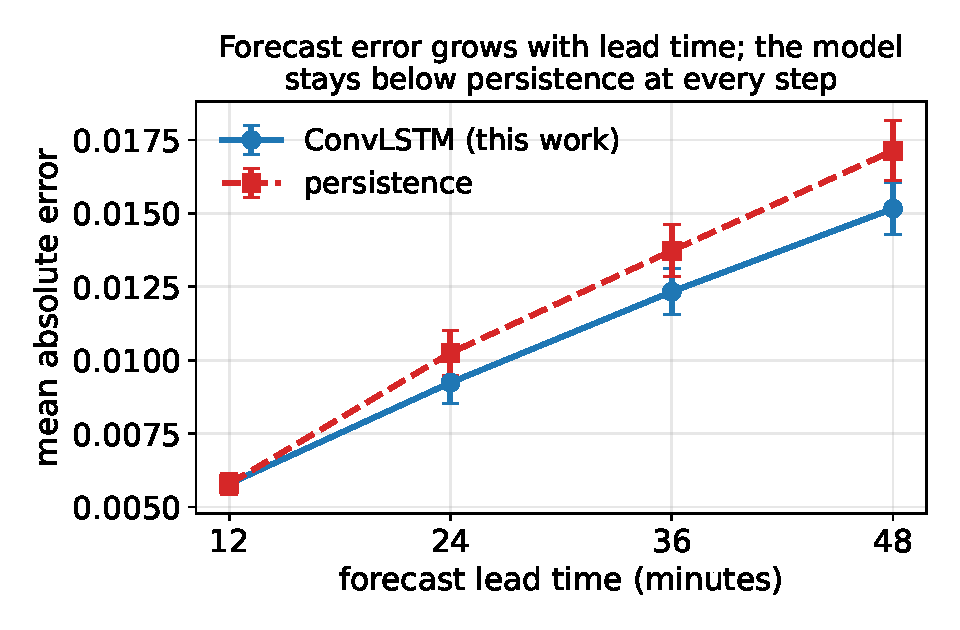
\includegraphics[width=0.66\textwidth]{figures/fig_skill_horizon.pdf}
\caption[Error vs.\ lead time]{\textbf{Forecast error versus lead time.} Mean
absolute error over all $61$ held-out windows for the ConvLSTM and for
persistence (error bars: standard error). The two coincide at $+12$~minutes and
diverge thereafter, the model staying below persistence at every subsequent step.}
\label{fig:horizon}
\end{figure}

\paragraph{Qualitative agreement across the sequence.}
Finally, Figure~\ref{fig:forecast} surveys three windows drawn from different days
across the held-out sequence, showing the input, the four forecasts, and the
observed frame. Sampled evenly, these span the range of per-window error (mean
absolute error from $0.028$ down to $0.007$); across all of them the large-scale
organisation of the winding field is reproduced over the full horizon.

\begin{figure}[t]
\centering
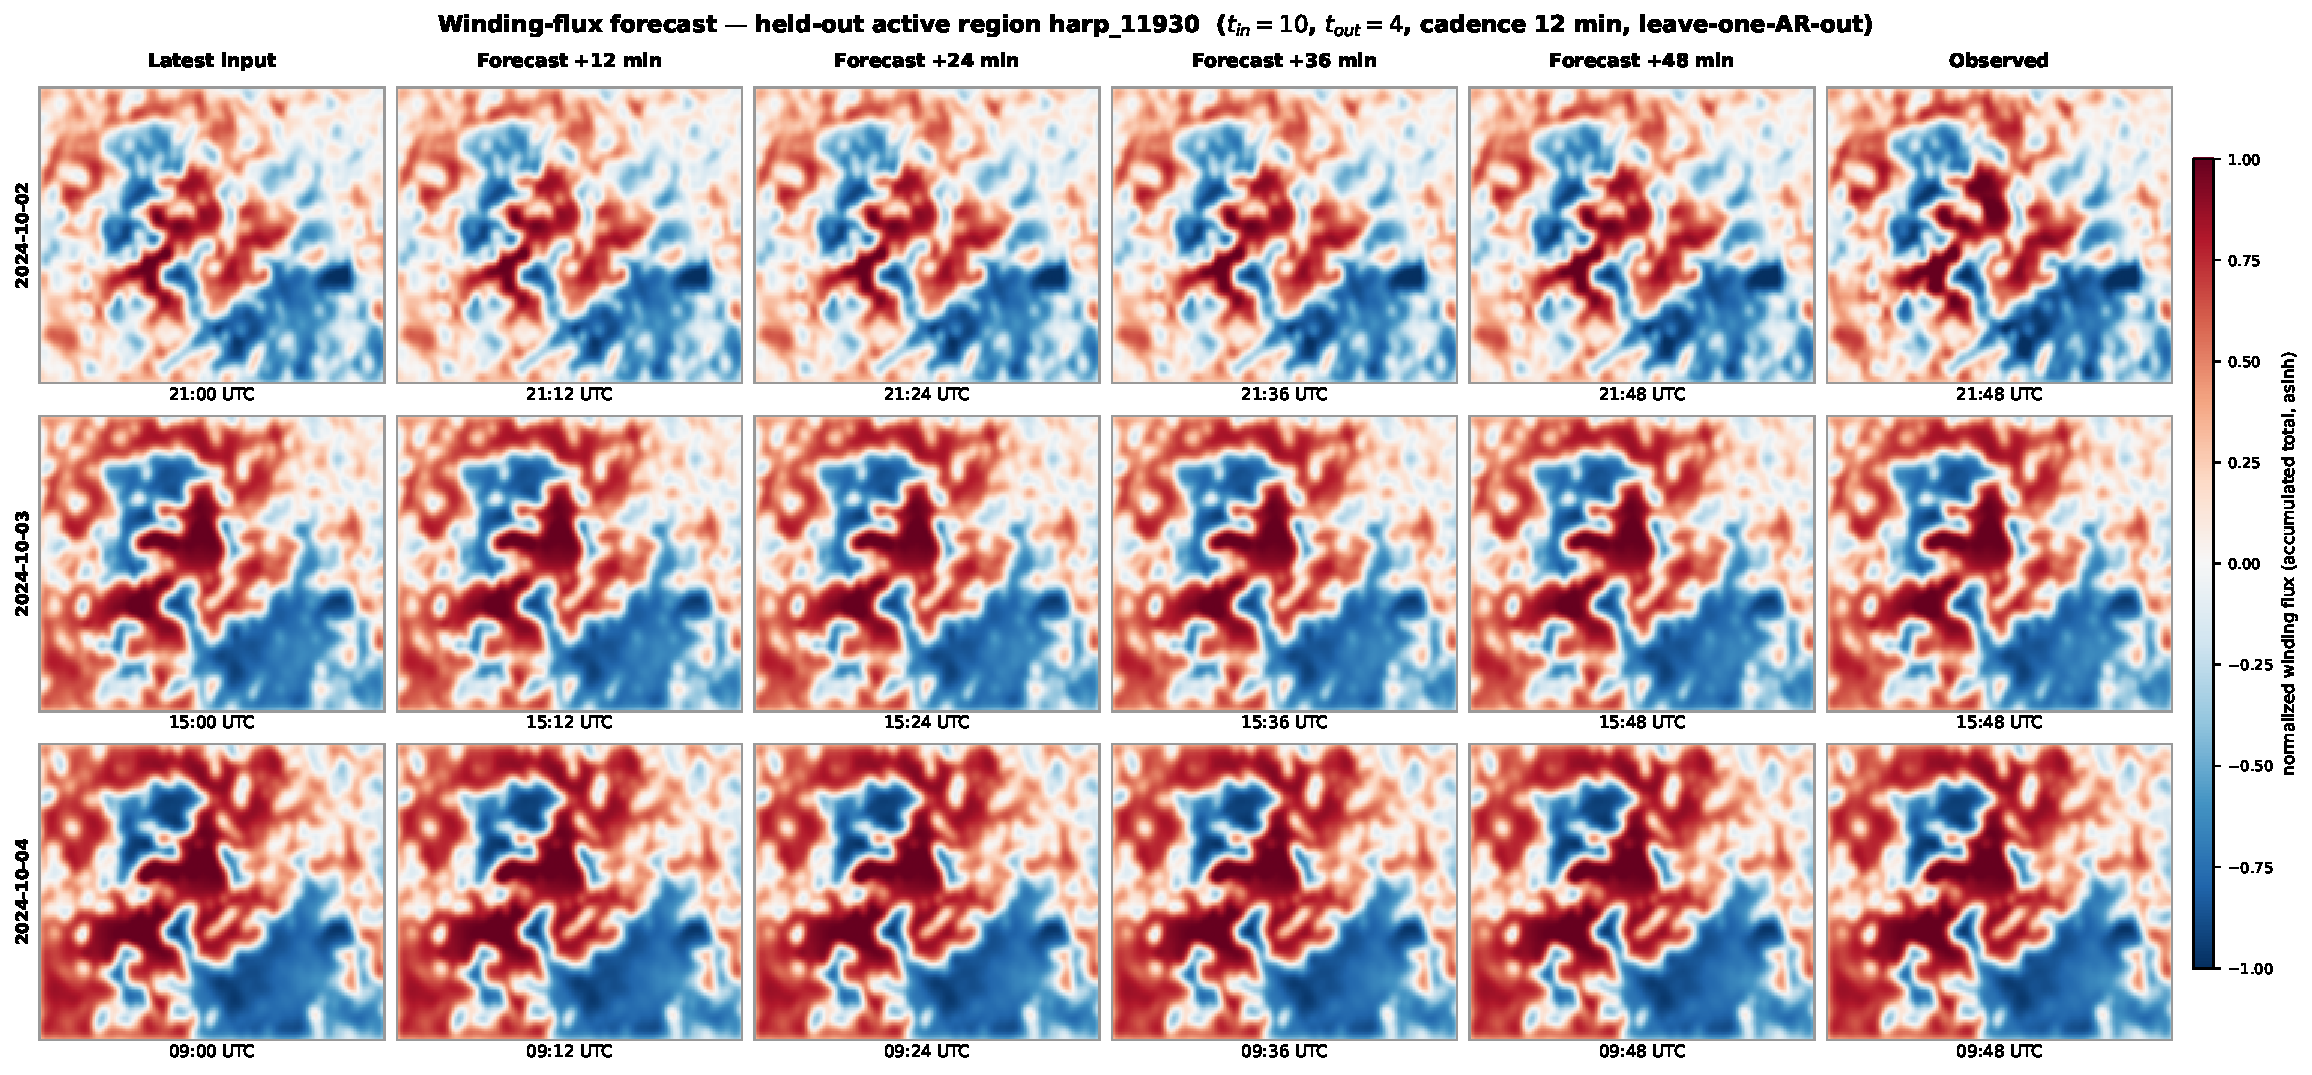
\includegraphics[width=\textwidth]{figures/fig_forecast_loo.pdf}
\caption[Held-out forecasts]{\textbf{Winding-flux forecasts on the held-out
active region HARP~11930.} Each row is an independent window: the latest input
frame, the four autoregressive forecasts at $+12,+24,+36,+48$~minutes, and the
observed frame at $+48$~minutes, all stamped with their true UTC time. The model
is trained only on the other $26$ regions.}
\label{fig:forecast}
\end{figure}

\section{Discussion}
\label{sec:discussion}

Three points must be made plainly, because the visual quality of
Figure~\ref{fig:forecast} is easy to over-read.

\paragraph{The skill is real but small, and persistence-dominated.}
The model beats persistence by $9.3\%$ on a held-out region, so it has learned
something transferable about how the winding field evolves, beyond copying.
But the margin is modest, and it must be. As established in \S\ref{sec:data} and
Figure~\ref{fig:autocorr}, the accumulated total winding builds up gradually and
is therefore strongly autocorrelated from frame to frame; persistence is already
a strong forecast, and there is limited headroom above it. The striking agreement
between prediction and observation in Figure~\ref{fig:forecast} is therefore in
large part a statement about the \emph{predictability of the total field}, and
the honest measure of what the model adds is the skill relative to persistence,
not the visual match. Quoting that baseline alongside every result is what keeps
the account truthful.

\paragraph{The forecastable content is the low-pass envelope.}
The spatial low-pass of \S\ref{sec:data} was applied deliberately, and the
result vindicates the reasoning behind it: what the model reproduces is the
large-scale envelope of the winding field, not its fine structure. The
small-scale detail that the low-pass removed evolves incoherently from frame to
frame and could not have been forecast in any case; excluding it lets the model
spend its capacity where skill is attainable. This is an honest restriction of
scope, not a hidden one.

\paragraph{Outlook.}
Taken together, the experiment delivers a working spatiotemporal pipeline for
two-dimensional winding-flux maps and a clear-eyed measurement of what such
forecasting can yield. The path from here is not a better frame predictor---the
persistence ceiling makes that a diminishing return---but the use of the learned
spatiotemporal representation for the task that motivated the winding map in the
first place: discriminating flare-productive from quiet configurations from the
structure the scalar integral throws away.
